\documentclass[a4paper]{article}

%use the english line for english reports
%\usepackage[english]{babel}
\usepackage[portuguese]{babel}
\usepackage[utf8]{inputenc}
\usepackage{indentfirst}
\usepackage{graphicx}
\usepackage{verbatim}
\usepackage{url}
\usepackage[a4paper, total={6in, 8in}]{geometry}

\begin{document}

\setlength{\textwidth}{16cm}
\setlength{\textheight}{22cm}

\title{\Huge\textbf{7th Guest: Infection}\linebreak\linebreak\linebreak
\Large\textbf{Relatório Final}\linebreak\linebreak
\linebreak\linebreak

\includegraphics[scale=0.1]{feup-logo.png}\linebreak\linebreak
\linebreak\linebreak
\Large{Mestrado Integrado em Engenharia Informática e Computação} \linebreak\linebreak
\Large{Programação em Lógica}\linebreak
}

\author{\textbf{Grupo 02:}\\ Diogo Machado - up201706832 \\ Eduardo Ribeiro - up201705421 \\\linebreak\linebreak \\
 \\ Faculdade de Engenharia da Universidade do Porto \\ Rua Roberto Frias, s\/n, 4200-465 Porto, Portugal \linebreak\linebreak\linebreak
\linebreak\linebreak\vspace{1cm}}
\maketitle
\thispagestyle{empty}



\newpage

\section*{Resumo}

\bigskip
Este trabalho consistiu no desenvolvimento do jogo \textbf{\textit{7th Guest: Infection}}, na linguagem de programação \textit{Prolog}.

\bigskip
Trata-se de um jogo disputado entre dois jogadores, numa grelha 7x7, e cujo vencedor é o jogador com mais peças no tabuleiro, no final do jogo. Podendo o computador controlar um dos jogadores, ou até ambos, existem assim três modos de jogo: Humano vs Humano, Humano vs Computador e Computador vs Computador.

\bigskip
Os principais objetivos para o projeto eram os de implementar com sucesso todas as regras do jogo, implementar com sucesso os três modos de jogo, implementar com sucesso diferentes níveis de dificuldade para os jogadores controlados pelo computador, e fazer tudo isto com um grau satisfatório de eficiência, em termos de desempenho.

\bigskip
Para a implementação do jogo, as diferentes tarefas foram distribuídas por diferentes módulos, cada um no seu ficheiro \textit{Prolog} (\textit{logic.pl}, \textit{boardManip.pl}, etc), de modo a que os predicados com funcionalidades relacionadas estivessem agrupados.

Seguindo esta organização, implementamos um ciclo de jogo com uma estrutura standard, no qual o estado de jogo é obtido, alterado e armazenado até que se verifique pelo menos uma das condições de fim de jogo.

\bigskip
Tendo permitido verificar a eficiência da linguagem \textit{Prolog} quando aplicada na resolução de problemas de decisão, um dos principais obstáculos à realização do projeto foi o facto de se tratar do primeiro contacto com esta, sendo que, quando se ultrapassou o período inicial de adaptação, o ritmo do desenvolvimento do projeto aumentou bastante.

\bigskip
Após a elaboração do projeto, julgamos ter conseguido cumprir os objetivos a que nos propusemos, sendo que conseguimos implementar todas as funcionalidades que eram pretendidas, sem grandes problemas de performance.
    
\newpage
\tableofcontents

\newpage

%%%%%%%%%%%%%%%%%%%%%%%%%%
\section{Introdução}

\bigskip
Este projeto foi desenvolvido no âmbito da unidade curricular de \textbf{Programação em Lógica}, do 3º Ano do Mestrado Integrado em Engenharia Informática e Computação da FEUP.

O projeto consiste na implementação do jogo de tabuleiro \textit{7th Guest: Infection}, no sistema \textit{SICStus Prolog}.

\bigskip
O trabalho teve como objetivo a aplicação da linguagem \textit{Prolog} na implementação do jogo, incluindo vários desafios como a implementação das regras específicas do jogo, ou o desenvolvimento de uma inteligência artificial a partir da qual é possível jogar contra o computador (ou até deixar o computador jogar contra si mesmo).

\bigskip
Este relatório reger-se-á pela seguinte estrutura:

\begin{itemize}
    \item \textbf{O Jogo - 7th Guest: Infection}: Descrição do jogo, incluindo uma breve apresentação da sua história e a descrição das regras
    \item \textbf{Lógica do Jogo}: Descrição da nossa implementação da lógica do jogo, tocando os seguintes aspetos:
    \begin{itemize}
        \item \textbf{Representação do Estado do Jogo}: Explicação de como o estado do jogo é representado na nossa implementação, com exemplos do estado inicial, de estados intermédios e de estados finais do jogo
        \item \textbf{Visualização do Tabuleiro}: Expliação do método implementado para a visualização do estado interno do jogo, por parte do utilizador
        \item \textbf{Lista de Jogadas Válidas}: Descrição do método implementado para a geração e validação de jogadas possíveis, para um dado ponto do jogo
        \item \textbf{Execução de Jogadas}: Explicação do modo como são processadas a validação e a execução das jogadas efetuadas pelos jogadores
        \item \textbf{Final do Jogo}: Descrição dos predicados que verificam (e, se caso disso, executam) o final do jogo
        \item \textbf{Avaliação do Tabuleiro}: Explicação do método utilizado para a comparação de diferentes estados do jogo, com base em quão vantajosos são para um dado jogador
        \item \textbf{Jogada do Computador}: Descrição do predicado que gera a jogada a ser efetuada pelo computador, a um dado ponto no jogo, com base no nível de dificuldade definido
    \end{itemize}
\end{itemize}

%%%%%%%%%%%%%%%%%%%%%%%%%%
\newpage\section{O Jogo - 7th Guest: Infection}
\bigskip
\subsection{História do Jogo}

\bigskip
“The 7th Guest: Infection” é um jogo abstrato de estratégia que originalmente apareceu como “Microscope Puzzle” no jogo de computador de 1993, “The 7th Guest”. É baseado na família Ataxx de jogos de tabuleiro, cuja linhagem começou com um jogo de computador  de 1988 chamado “Infection”. 

\bigskip
A primeira versão deste jogo foi feita em 1988 por Wise Owl software. Escrito por Dave Crummack e Craig Galley, “Infection” foi programado nas consolas “Amiga”, “Commodore 64” e “Atari ST”. Os direitos do jogo foram vendidos à Leland Corporation, que lançou o jogo com o nome de “Ataxx”.

\bigskip
Em 1993, Trilobyte lançou “The 7th Guest”, que incluía uma versão deste jogo. Quando Trilobyte re-lançou “The 7th Guest” para o iPhone e iPad em 2010, anunciaram que alguns puzzles, incluíndo o “Microscope Puzzle”, não seriam incluídos devido a dificuldades técnicas associadas com a adaptação do jogo original às novas plataformas. No entanto, depois de o jogador completar o jogo, é possível acederem à versão antiga de “Infection”; o puzzle pode então ser jogado através deste método.

\bigskip
Uma versão atualizada do “Microscope Puzzle” foi lançada para o iPad com o nome de “The 7th Guest: Infection”, em Abril de 2011.

\bigskip
\begin{figure}[hbp!]
    \centering
    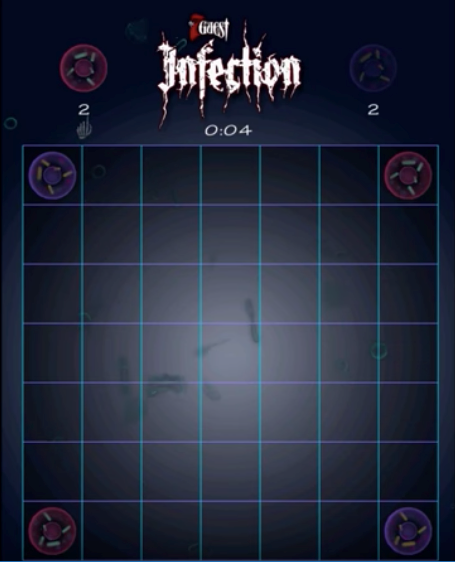
\includegraphics[width=.55\linewidth]{others/game-1.png}
    \caption{Ecrã inicial do jogo}
    \label{fig}
\end{figure}

\newpage\subsection{Regras do Jogo}

\bigskip
\begin{itemize}
    \item O tabuleiro é uma grelha quadrada com \textbf{7 linhas e 7 colunas}.
    \item Cada jogador começa com \textbf{dois micróbios}, de cor azul ou vermelha. Os micróbios são colocados nos \textbf{quatro cantos do tabuleiro}, sendo que os micróbios azuis ficam nos cantos superior esquerdo e inferior direito, e os vermelhos ficam nos outros 2 cantos. O \textbf{primeiro turno} é do jogador controlando os \textbf{micróbios vermelhos}.
    \item Durante um turno, um jogador pode \textbf{mover} um dos seus micróbios \textbf{uma ou duas casas} em \textbf{qualquer direção}, \textbf{incluindo diagonalmente}.
    \item Se um micróbio avançar \textbf{uma casa}, um \textbf{novo micróbio} (da mesma cor) é criado no espaço que o micróbio abandonou.
    \item Se um micróbio avançar \textbf{duas casas}, o espaço onde o micróbio começou o turno \textbf{fica vazio}.
    \item Ao movimentar um micróbio, todos os \textbf{micróbios do oponente} que estão \textbf{adjacentes} ficam \textbf{\textit{“infetados”}}, ficando com a cor do jogador que se movimentou.
    \item Os jogadores são \textbf{obrigados a fazer um movimento} a menos que nenhum movimento legal seja possível. 
    \item O jogo acaba quando se verifica uma das seguintes condições:
    \begin{itemize}
        \item \textbf{todos os espaços do tabuleiro estão preenchidos}
        \item \textbf{todos os micróbios em campo são de uma cor}
    \end{itemize}
    O jogador com \textbf{mais micróbios} em campo no fim do jogo é o vencedor!

\end{itemize}

\bigskip
\begin{figure}[hbp!]
    \centering
    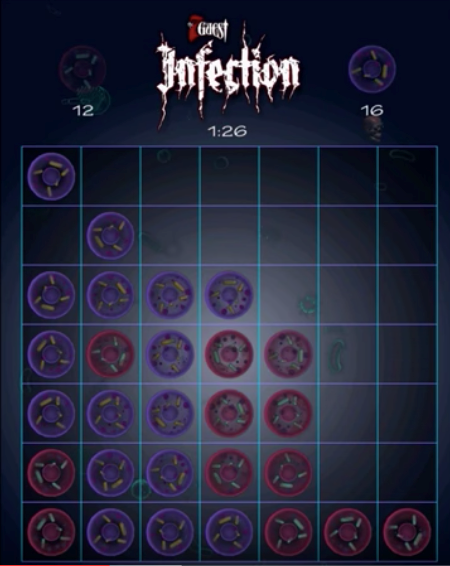
\includegraphics[width=.4\linewidth]{others/game-2.png}
    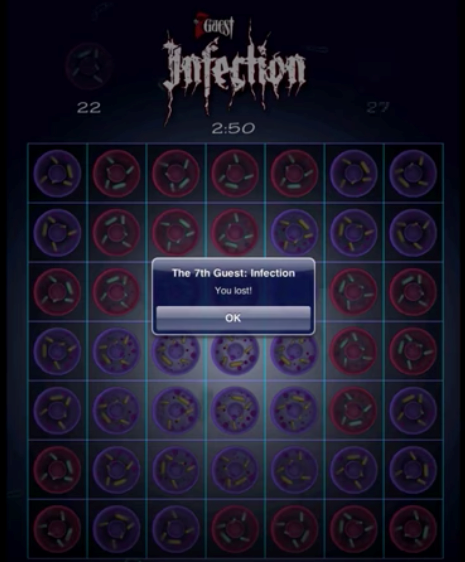
\includegraphics[width=.416\linewidth]{others/game-3.png}
    \caption{Exemplos do jogo}
    \label{fig}
\end{figure}

%%%%%%%%%%%%%%%%%%%%%%%%%%
\newpage\section{Lógica do Jogo}

Irá ser descrita nesta secção a nossa implementação do jogo em Prolog, falando sobre diferentes tópicos desde a visualização do estado de jogo até ao cálculo e geração de jogadas do computador.

\bigskip
O predicado principal do jogo é denominado \textbf{play}. Este inicializa o estado do jogo e começa-o (\textbf{startGame}), e depois contém o ciclo principal do jogo. Este é formado por 3 tarefas principais: \textbf{getState}, que extrai o estado de jogo atual, \textbf{changeState}, que gera uma jogada e modifica o estado de jogo, e \textbf{saveState}, que tendo em conta essa mudança guarda o estado de jogo modificado, para a próxima iteração do ciclo. Os predicados built-in \textbf{repeat} e \textbf{once} são utilizados de modo a criar um ciclo, sendo que cada iteração caracteriza um turno/jogada. 

\bigskip
O predicado \textbf{game\_over} é também chamado em cada iteração, sendo verdadeiro apenas se a condição de terminação do jogo foi alcançada; se este for o caso, é executada a saída do ciclo de jogo, e é chamado o predicado \textbf{showWinnerAndReset}, que mostra o vencedor do jogo (ou se houve empate), e que restabelece os valores iniciais do estado de jogo, para a próxima vez que o predicado play for executado.
\bigskip

\begin{figure}[hbp!]
    \centering
    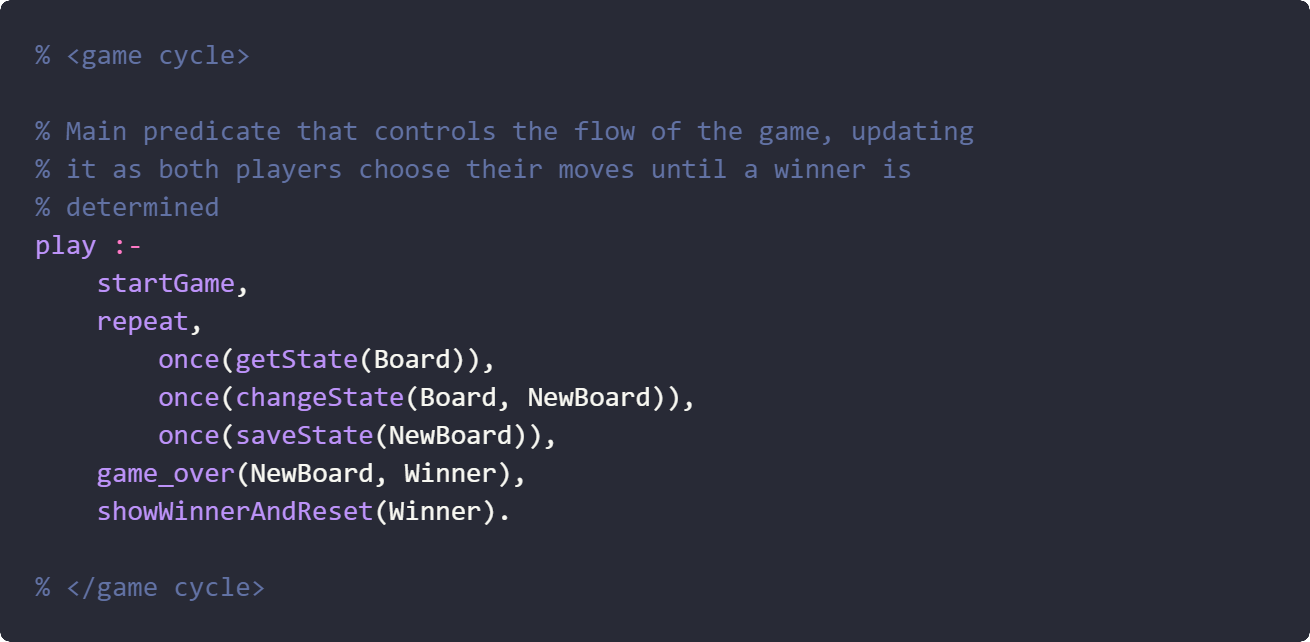
\includegraphics[width=\linewidth]{prints/play-cycle.png}
    \caption{Ciclo principal do jogo}
    \label{fig}
\end{figure}

\newpage\subsection{Representação do Estado do Jogo} 

\bigskip
O tabuleiro de jogo, de dimensões 7x7, é representado por uma lista (I) de listas (II), sendo que cada lista (II) representa uma fila do tabuleiro. Dentro de cada lista (II), existem 7 átomos, que podem tomar os valores ‘a’, ‘b’, ou ‘ ’, que representam, respetivamente, peças do Jogador A, do Jogador B, e espaços vazios no tabuleiro.

\bigskip
O estado inicial do jogo, como exibido na imagem acima, inclui duas peças do Jogador A, nos cantos superior esquerdo e inferior direito, e duas peças do Jogador B, nos cantos superior direito e inferior esquerdo, e o resto do tabuleiro vazio, sendo este estado internamente representado no seguinte formato:

\bigskip
\begin{figure}[hbp!]
    \centering
    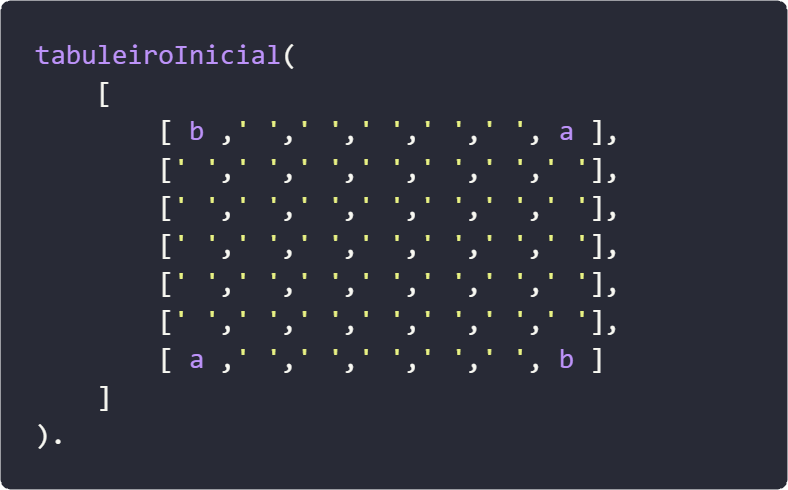
\includegraphics[width=.599\linewidth]{prints/game-tab-inicial.png}
    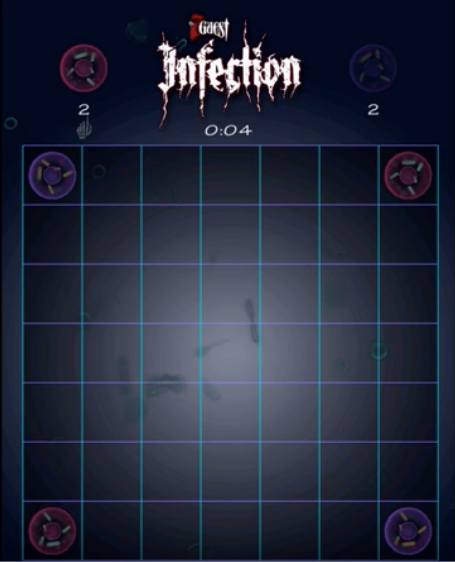
\includegraphics[width=.301\linewidth]{others/game-tab-inicial.png}
    \caption{Estado inicial do jogo}
    \label{fig}
\end{figure}

\bigskip
Um estado intermédio do jogo incluirá várias peças no tabuleiro, não se verifican-do ainda nenhuma das condições de final do jogo:

\bigskip
\begin{figure}[hbp!]
    \centering
    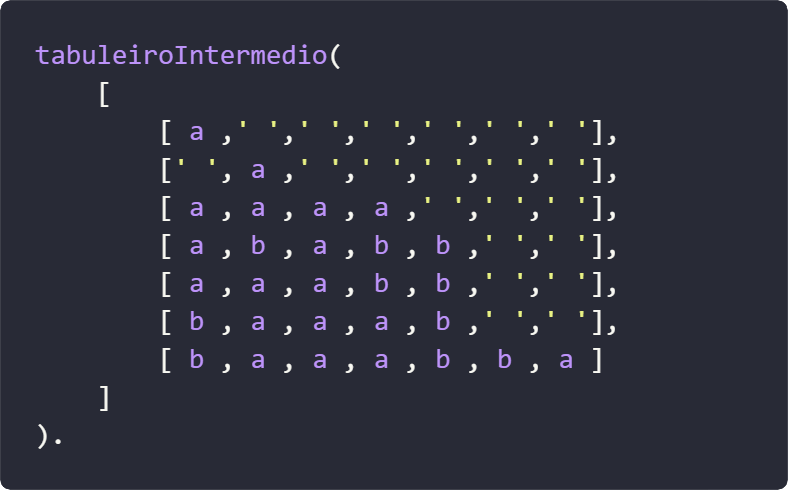
\includegraphics[width=.603\linewidth]{prints/game-tab-interm.png}
    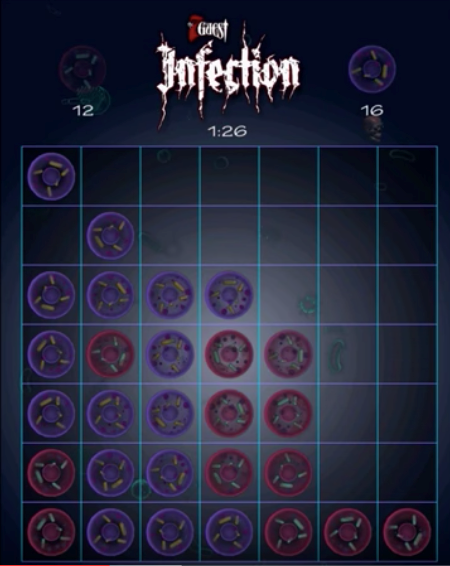
\includegraphics[width=.297\linewidth]{others/game-tab-interm.png}
    \caption{Possível estado intermédio do jogo}
    \label{fig}
\end{figure}

\newpage
\textbf{O estado final do jogo pode ser atingido a partir de três condições}:

\begin{itemize}
    \item Todas as peças do tabuleiro pertencem ao Jogador A.
    \begin{figure}[hbp!]
        \centering
        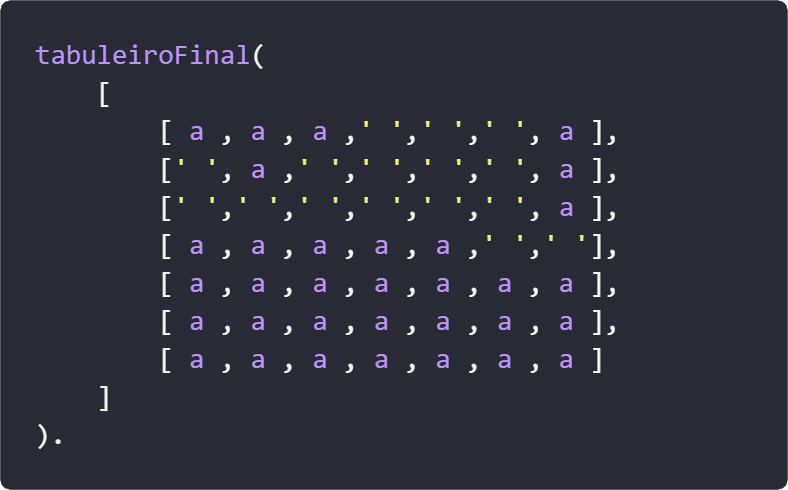
\includegraphics[width=.6\linewidth]{prints/game-tab-final-1.png}
    \end{figure}
    \item Todas as peças do tabuleiro pertencem ao Jogador B.
    \begin{figure}[hbp!]
        \centering
        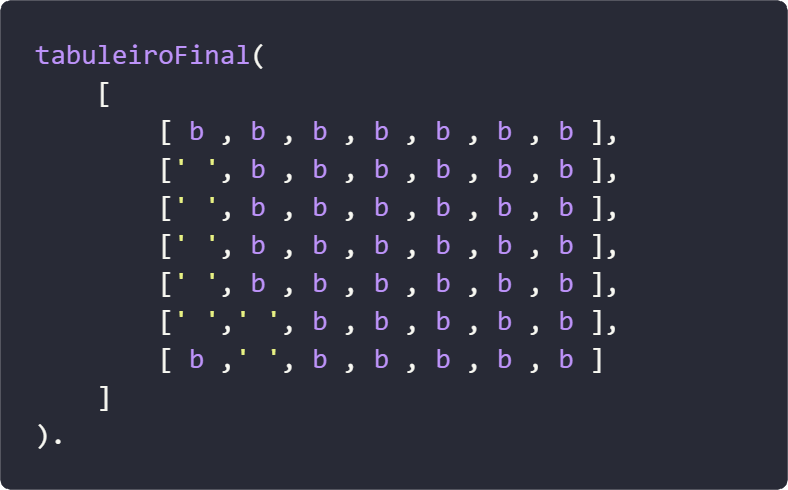
\includegraphics[width=.6\linewidth]{prints/game-tab-final-2.png}
    \end{figure}
    \item O tabuleiro encontra-se completamente preenchido.
    \begin{figure}[hbp!]
        \centering
        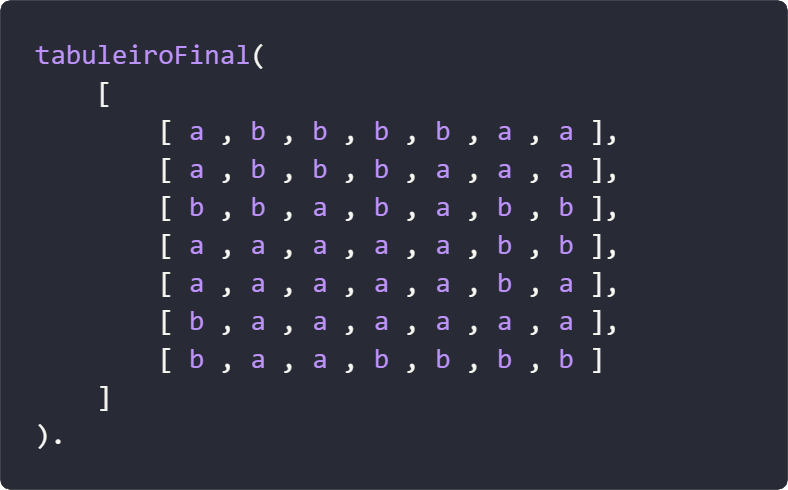
\includegraphics[width=.5945\linewidth]{prints/game-tab-final-3.png}
        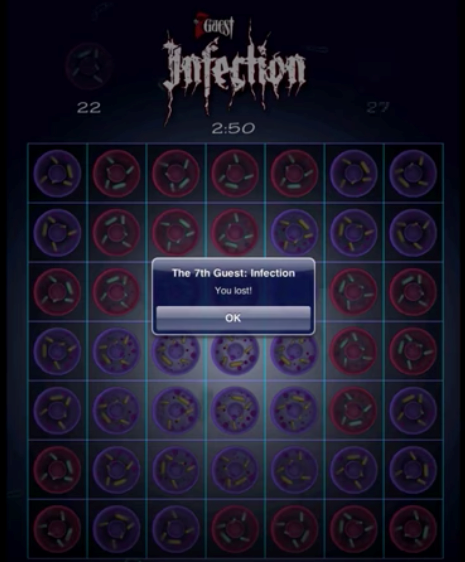
\includegraphics[width=.3055\linewidth]{others/game-tab-final.png}
    \end{figure}
\end{itemize}

\newpage\subsection{Visualização do Tabuleiro (\textit{display\_game})} 

\bigskip
O predicado utilizado para a visualização do tabuleiro percorre a \textbf{lista de listas} que descreve o estado do jogo, mostrando em seguida o número de pontos (peças no tabuleiro) de cada jogador. É indicado também indicado qual dos dois jogadores vai jogar a seguir.

\bigskip
\begin{figure}[hbp!]
    \centering
    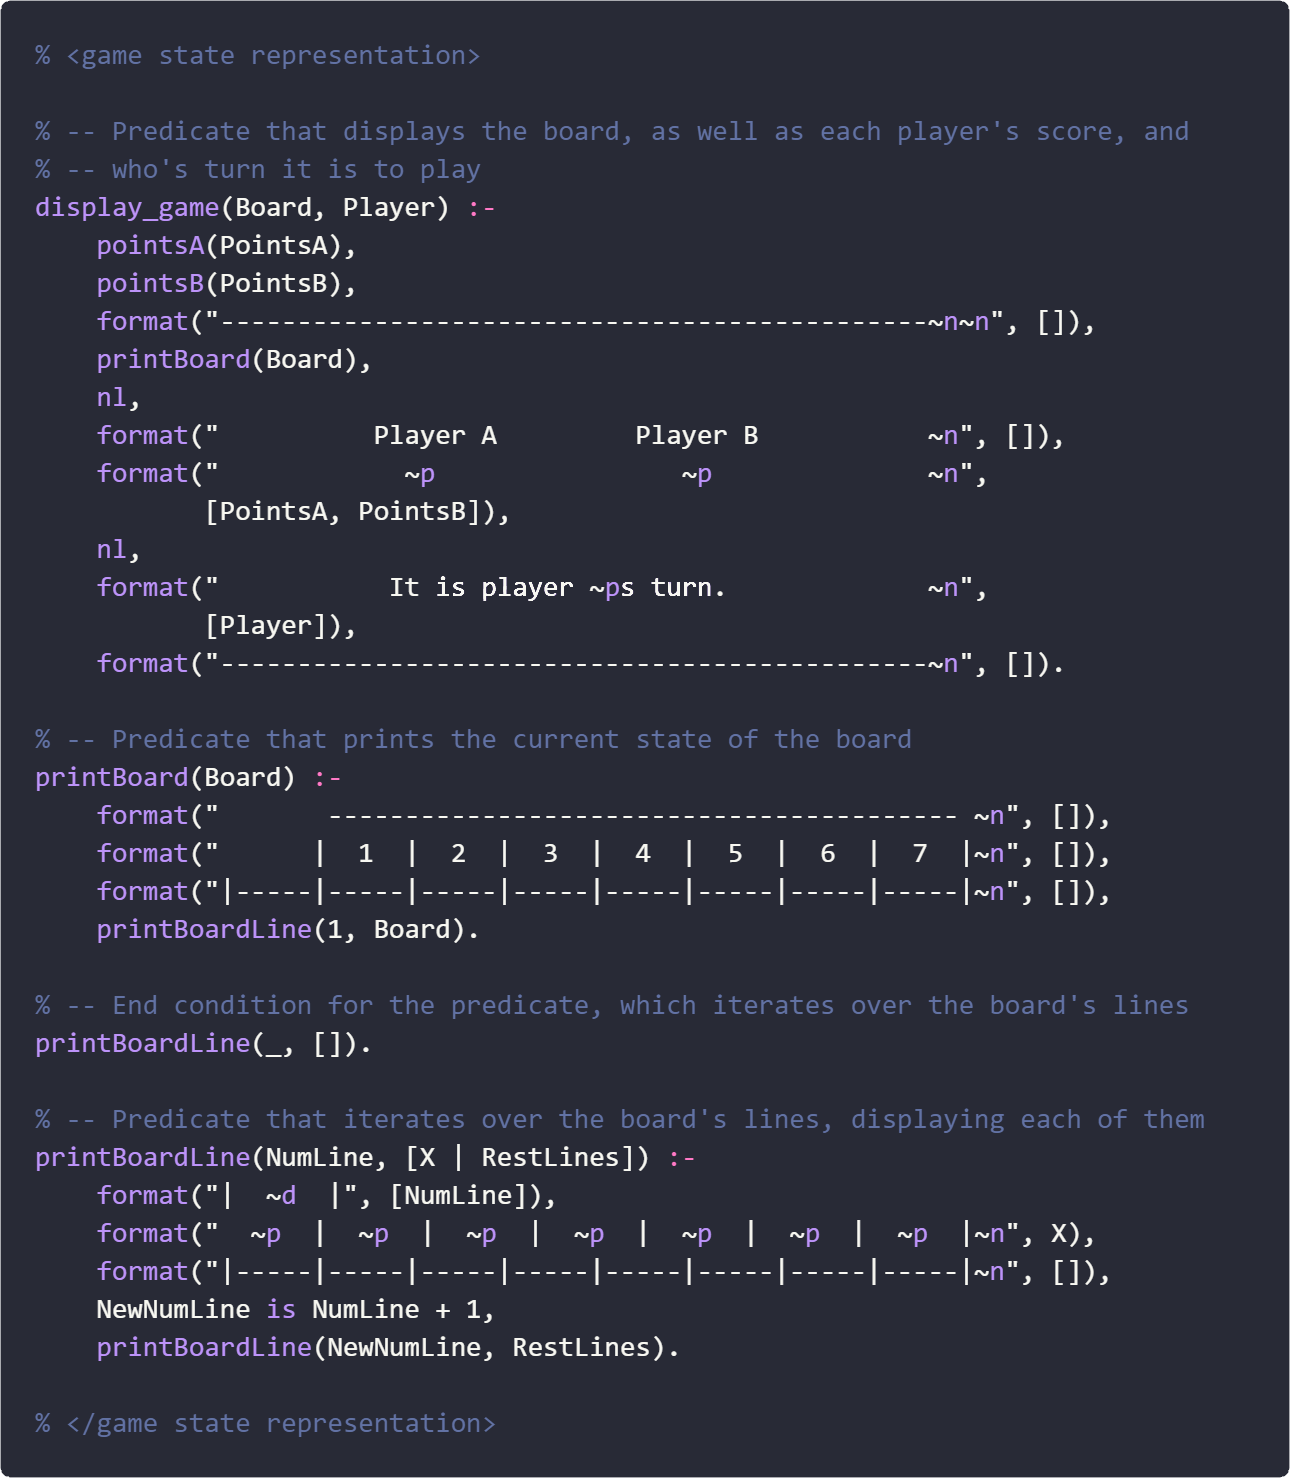
\includegraphics[width=\linewidth]{prints/game-representation.png}
    \caption{Código que apresenta o tabuleiro}
    \label{fig}
\end{figure}

\newpage
\begin{figure}[hbp!]
    \centering
    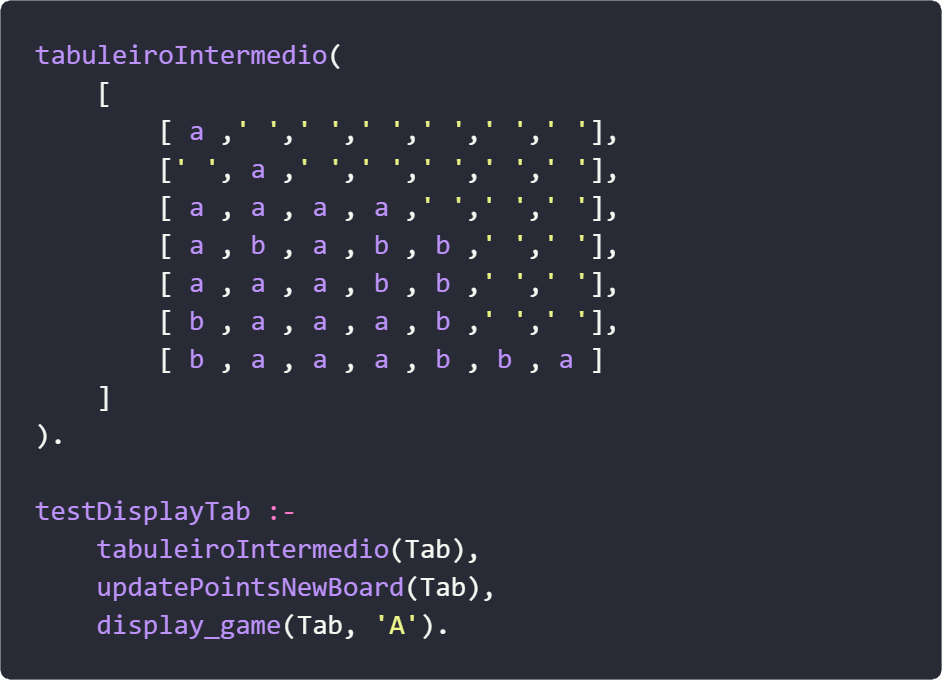
\includegraphics[width=.65\linewidth]{prints/test-tabuleiro.png}
    \caption{Predicado de teste da visualização do jogo}
    \label{fig}
\end{figure}

\begin{figure}[hbp!]
    \centering
    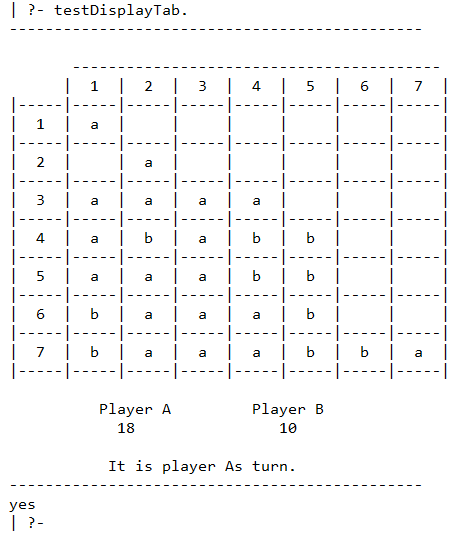
\includegraphics[width=.65\linewidth]{others/test-tabuleiro.png}
    \caption{Output do teste da visualização do jogo}
    \label{fig}
\end{figure}

\newpage\subsection{Lista de Jogadas Válidas (\textit{valid\_moves})}

\bigskip
O predicado em questão recebe uma variável denominada \textbf{Player}, que pode ser ‘A’ ou ‘B’, representando o jogador que deve jogar a seguir; uma variável chamada \textbf{Board}, contém o estado atual do jogo (tabuleiro); e retorna \textbf{ListOfValidMoves}, uma lista de estruturas que representam um dado movimento que o jogador poderá efetuar (são tuplos do género \textbf{OldLine-OldColumn-NewLine-NewColumn}, sendo que as variáveis \textbf{Old} se referem ao sítio onde a peça se encontrava, e as variáveis \textbf{New} à nova posição que a peça irá ter). Este predicado é utilizado na lógica das jogadas do computador, de modo a gerar todas as jogadas possíveis de modo a escolher a mais vantajosa, e também na lógica das jogadas do humano, de modo a saber se há alguma jogada válida que este poderá fazer (sendo que, se não existir, o seu turno é passado à frente).

\bigskip
O predicado utiliza o predicado built-in \textbf{findall}, que chama um predicado feito por nós denominado \textbf{findMove}. Este último retorna uma possível jogada que o \textbf{Player} poderá fazer, sendo que se o utilizador pedir outra solução (com ponto e vírgula), o predicado irá gerar outra jogada possível (se existir). Desta maneira, utilizando \textbf{findall} é possível gerar todas as jogadas válidas possíveis.

\bigskip
Relativamente ao funcionamento do predicado \textbf{findMove}, este, tendo em conta o jogador atual a jogar, tenta encontrar uma peça do mesmo que esteja no tabuleiro, gerando depois um possível movimento para essa peça (por exemplo, 1 casa para a esquerda). De seguida, verifica-se a validade dessa jogada, chamando o predicado \textbf{checkValidMove}, de modo ao predicado apenas ser verdadeiro se o movimento for válido, tendo em conta o conteúdo do tabuleiro atual. Com a estratégia adotada de gerar uma solução e de seguida verificar a validade da mesma, tira-se partido do mecanismo de retrocesso do Prolog, uma vez que, se o movimento não for válido, o retrocesso faz com que se escolha outro movimento e/ou outra peça do tabuleiro para mover (se for possível). O \textbf{once} é utilizado quando se chama \textbf{checkValidMove} de modo a evitar retrocesso dentro deste predicado.

\bigskip
\begin{figure}[hbp!]
    \centering
    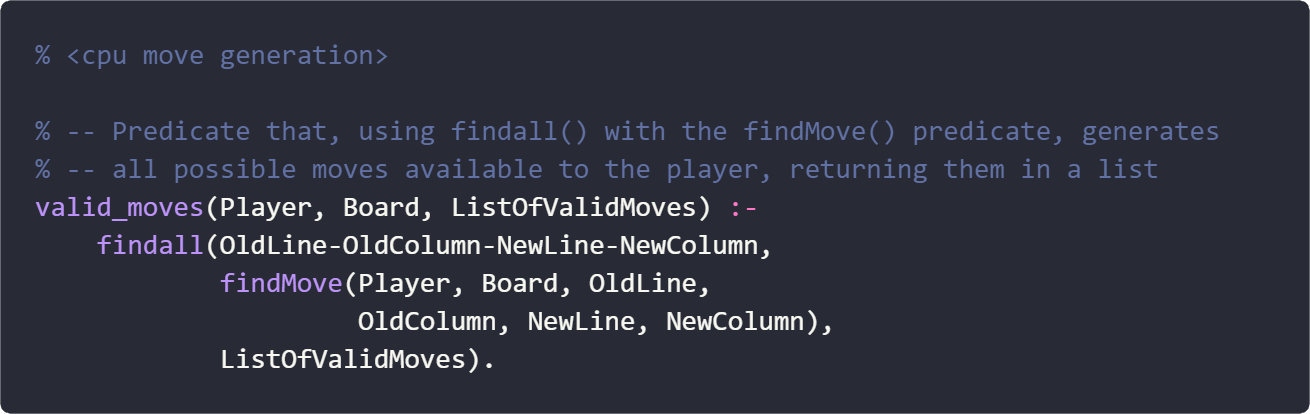
\includegraphics[width=\linewidth]{prints/move-generation-1.png}
    \caption{Código que gera as possíveis jogadas de um jogador}
    \label{fig}
\end{figure}

\newpage
\begin{figure}[hbp!]
    \centering
    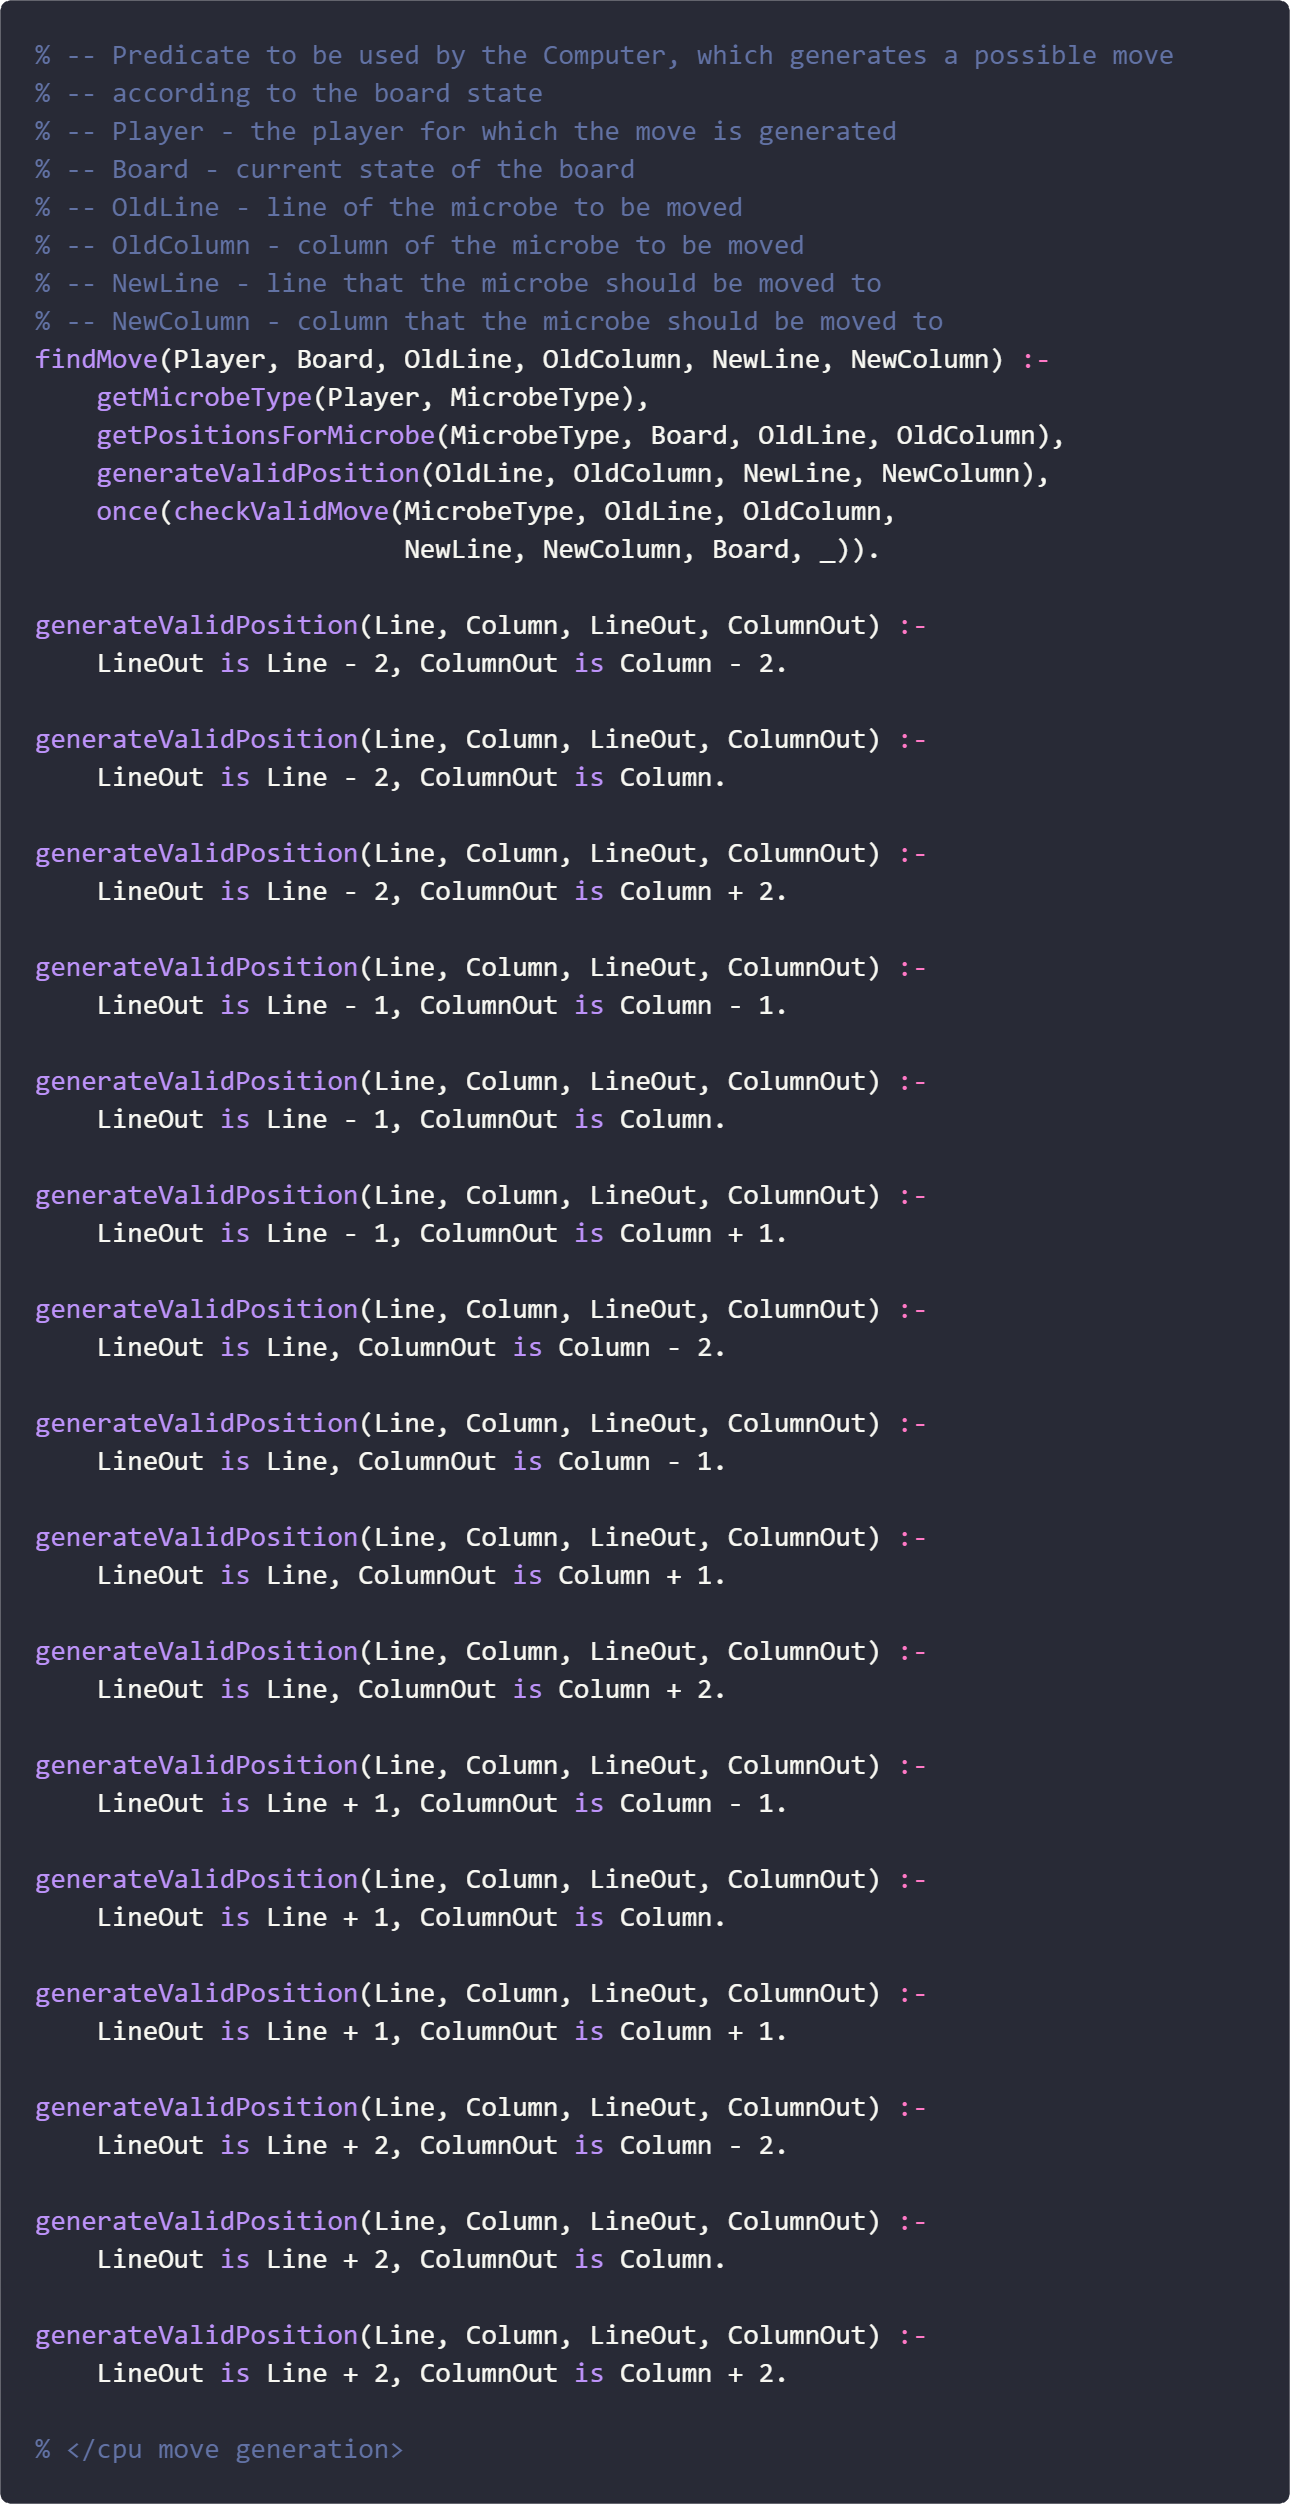
\includegraphics[width=.7\linewidth]{prints/move-generation-2.png}
    \caption{Predicado para encontrar uma potencial jogada para um jogador}
    \label{fig}
\end{figure}

\newpage\subsection{Execução de Jogadas (\textit{move})} 

\bigskip
O predicado \textbf{move} recebe: \textbf{Player}, que indica o jogador que está a fazer o movimento; a posição da peça que este pretende mover, através dos argumentos \textbf{OldLine} e \textbf{OldColumn}; a posição para a qual se pretende mover a peça, com \textbf{NewLine} e \textbf{NewColumn}; e \textbf{Board}, representando o tabuleiro atual. O predicado valida o movimento proposto pelo jogador, e se este for válido então o predicado modifica o tabuleiro, executando o movimento, sendo que o tabuleiro resultante é retornado através do argumento \textbf{NewBoard}. 

\bigskip
O predicado começa por saber qual é o tipo de peça que corresponde ao jogador, através de \textbf{getMicrobeType}. De seguida, chama \textbf{checkValidMove} de modo a verificar se o movimento proposto pelo jogador é valido; este predicado verifica se há uma peça do jogador na posição inicial, se a posição final se encontra livre, e se o movimento entre as duas posições é válido.

\bigskip
Se o movimento for válido, é adicionada uma nova peça na posição final (\textbf{playMicrobe}), sendo que a peça original é retirada se o movimento não for adjacente, e mantida caso seja (\textbf{handleIsAdjacent}). Por fim, chama um predicado que “contamina” todas as peças do oponente que são adjacentes à nova peça, que passam a ser peças do jogador que fez o movimento (\textbf{contaminateAdjacent}).

\bigskip
\begin{figure}[hbp!]
    \centering
    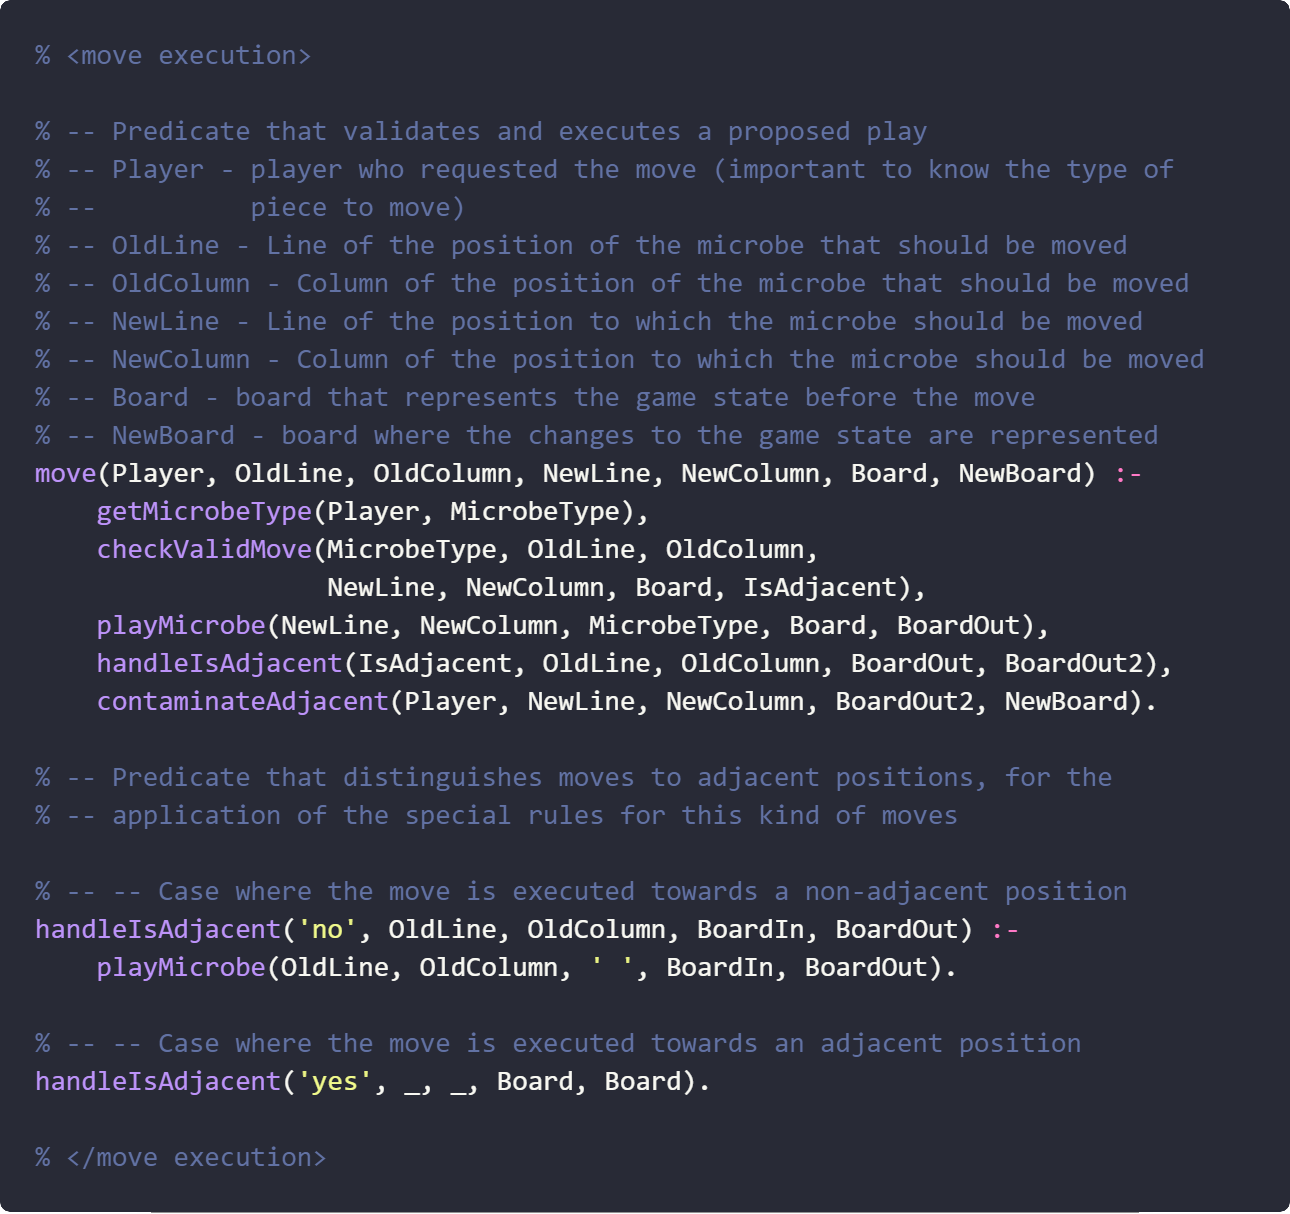
\includegraphics[width=.87\linewidth]{prints/move-execution.png}
    \caption{Código que valida e executa uma jogada}
    \label{fig}
\end{figure}

\newpage
\begin{figure}[hbp!]
    \centering
    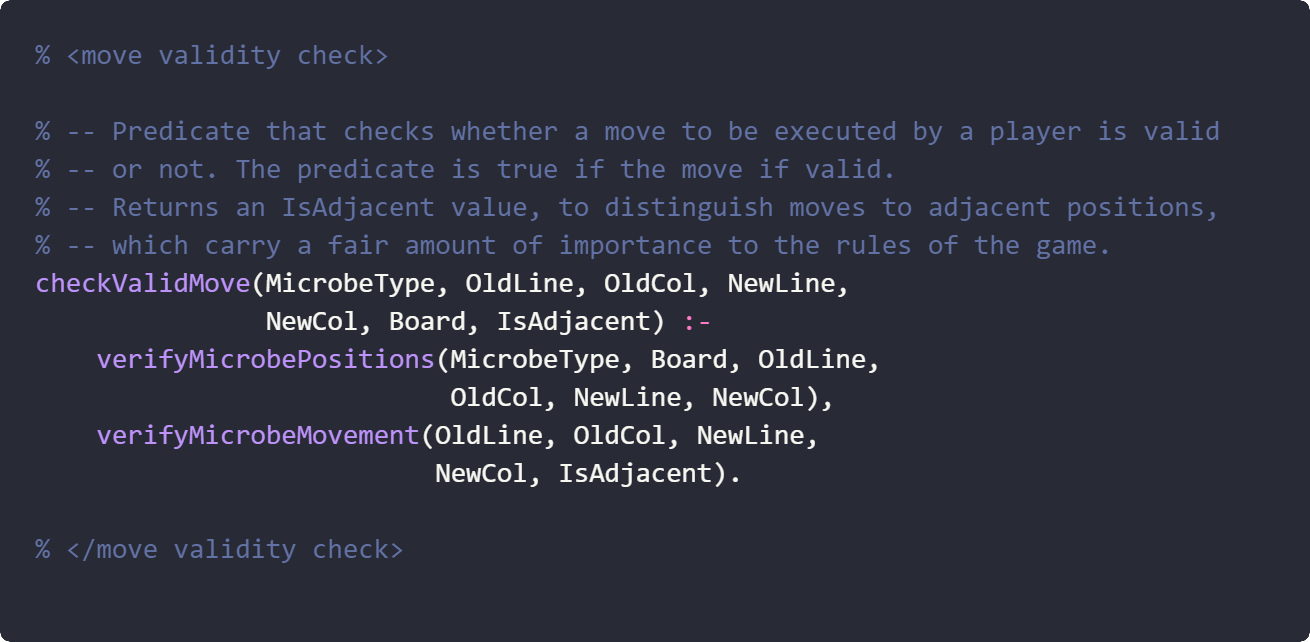
\includegraphics[width=.66\linewidth]{prints/move-validation.png}
    \caption{Validação de uma qualquer jogada}
    \label{fig}
\end{figure}

\begin{figure}[hbp!]
    \centering
    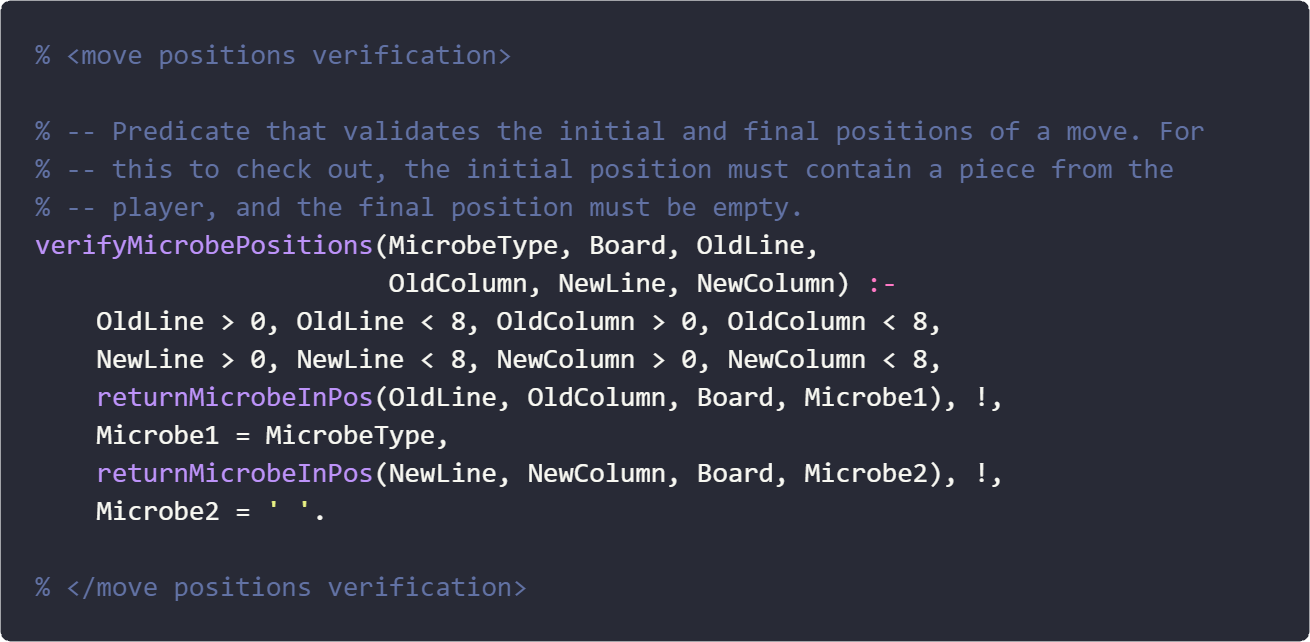
\includegraphics[width=.66\linewidth]{prints/move-position-verification.png}
    \caption{Verificação da posição para a qual a peça é movida}
    \label{fig}
\end{figure}

\begin{figure}[hbp!]
    \centering
    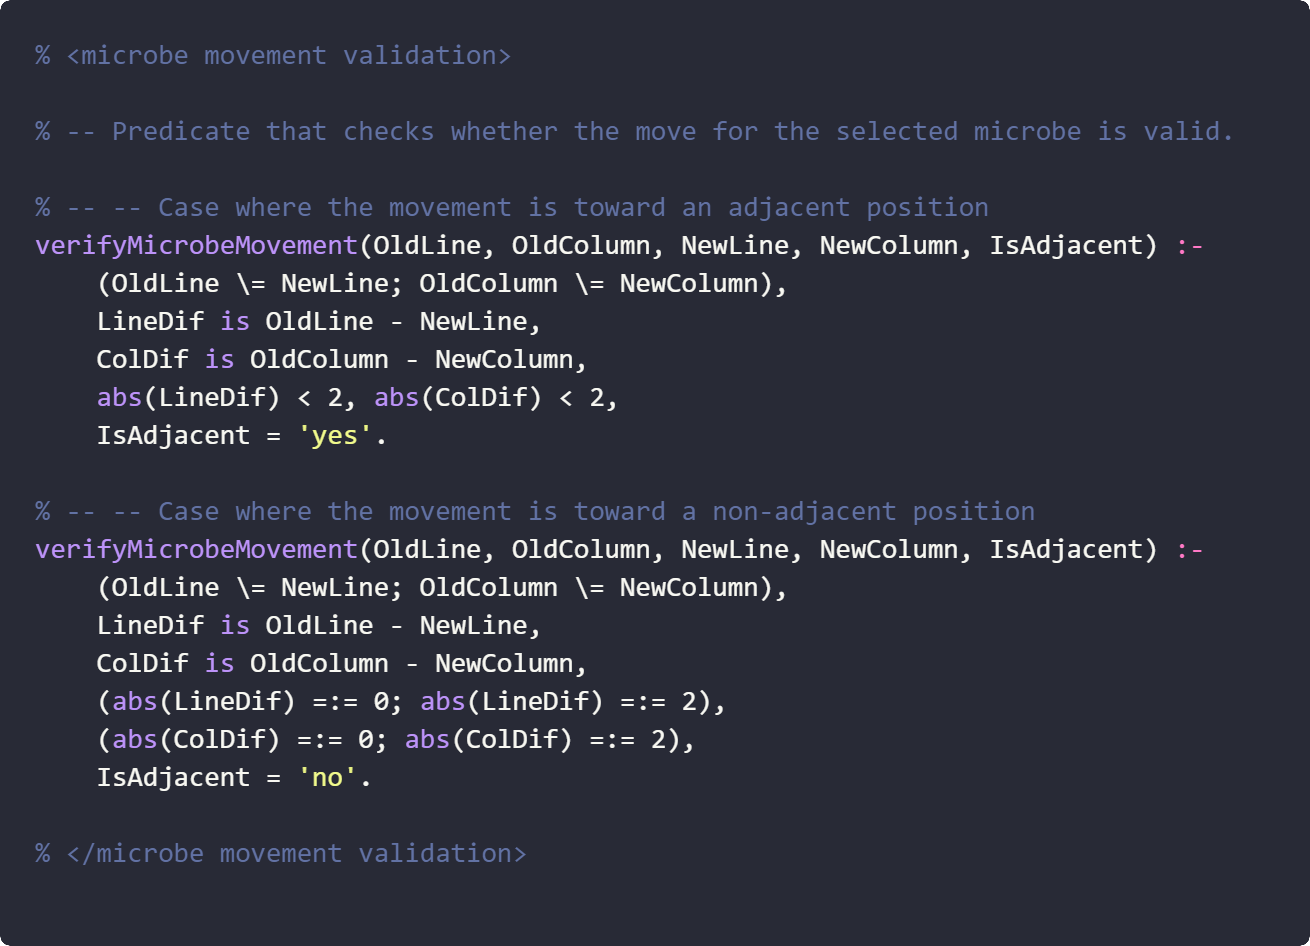
\includegraphics[width=.66\linewidth]{prints/move-movement-verification.png}
    \caption{Verificação da direção do movimento}
    \label{fig}
\end{figure}

\begin{figure}[hbp!]
    \centering
    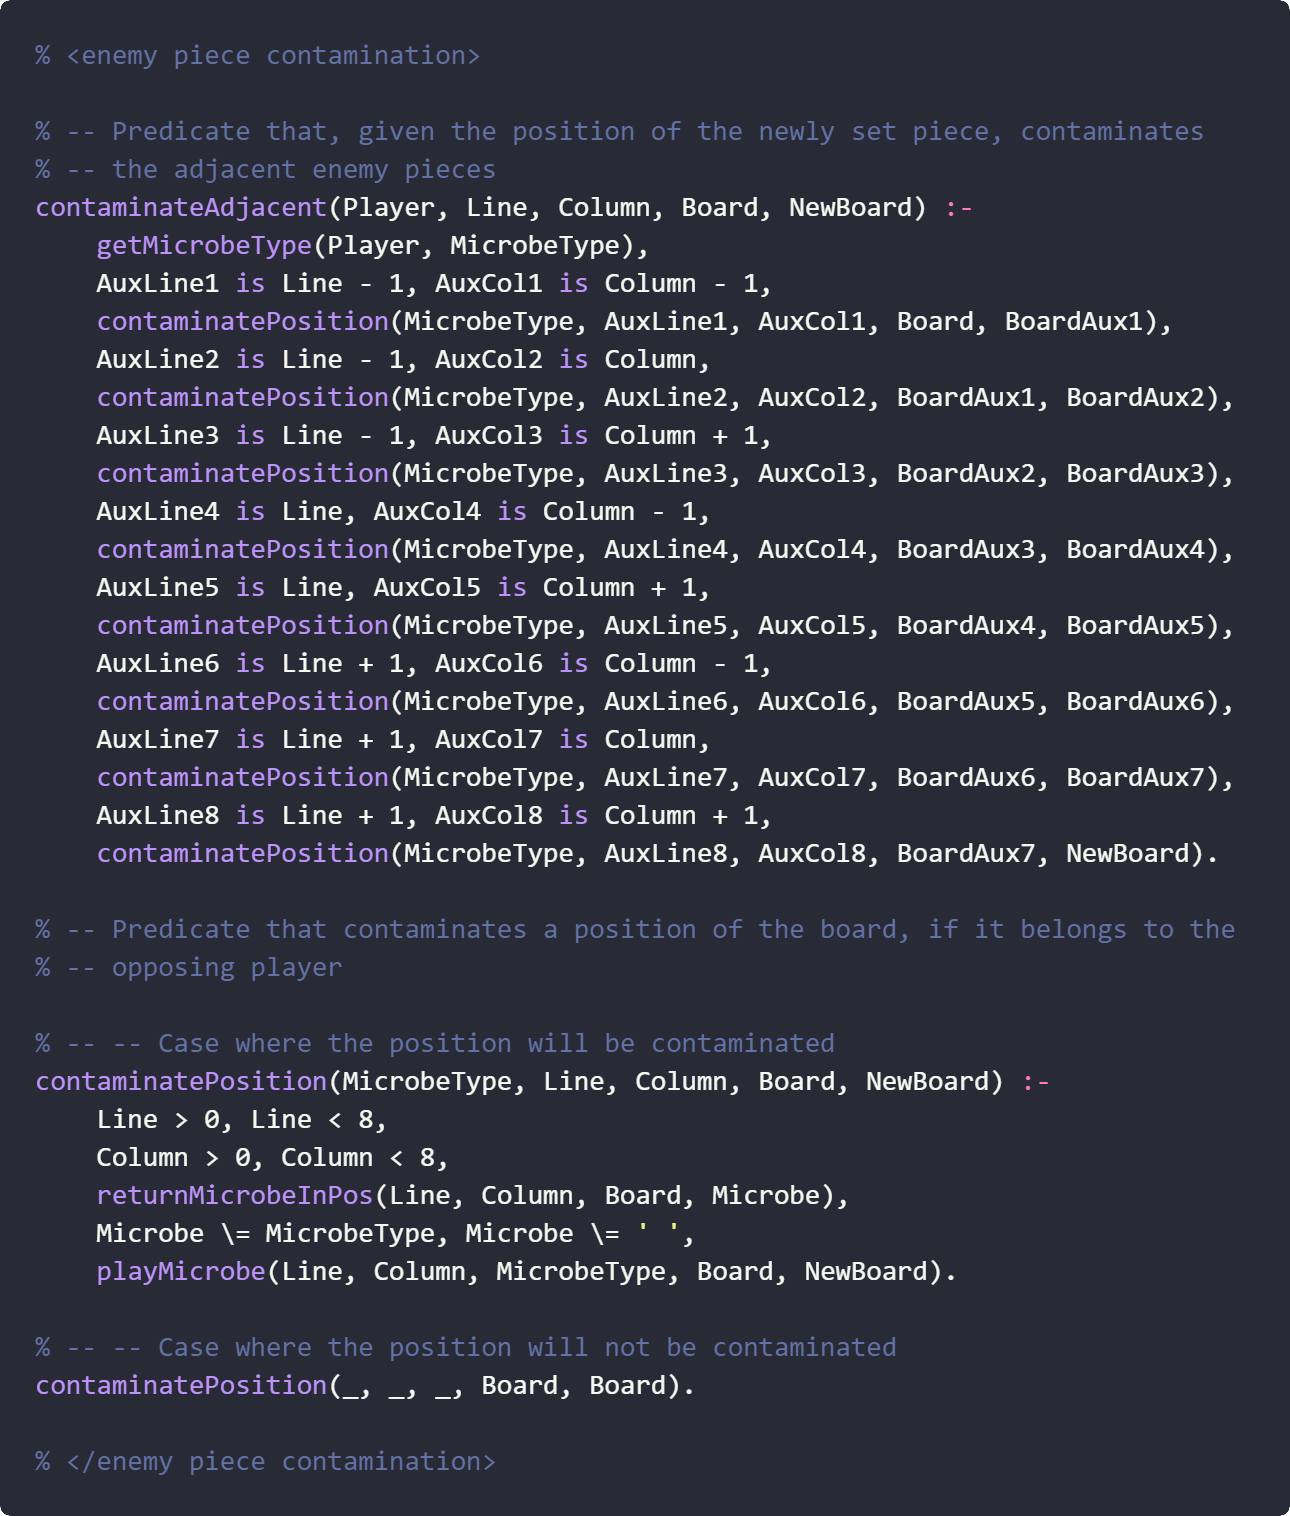
\includegraphics[width=\linewidth]{prints/move-enemy-contamination.png}
    \caption{Contaminação das peças inimigas adjacentes}
    \label{fig}
\end{figure}

\newpage\subsection{Final do Jogo (\textit{game\_over})} 

\bigskip
Este predicado recebe o estado atual do jogo, através de \textbf{Board}, verifica se o jogo acabou e, se tal ocorreu, identifica qual o jogador que venceu o jogo, retornando-o através de \textbf{Winner}.

\bigskip
Como descrito anteriormente, o jogo termina se apenas existem peças de um tipo em campo, ou se todas as posições do campo estão preenchidas, sendo que neste caso o vencedor é quem tem o maior número de peças no tabuleiro.

\bigskip
O predicado começa por percorrer o tabuleiro, verificando se existem peças do jogador B (se não houver, o vencedor é A). Verifica depois se existem peças do jogador A (se não houver, o vencedor é B). Por fim, verifica se existem espaços livres no tabuleiro. Caso esta última condição não seja verdadeira, o predicado compara o número de pontos atual de cada jogador, sendo que o vencedor é quem tem a pontuação mais alta (uma vez que o número de pontos de um jogador é igual ao número de peças que este tem em campo). 

\bigskip
\begin{figure}[hbp!]
    \centering
    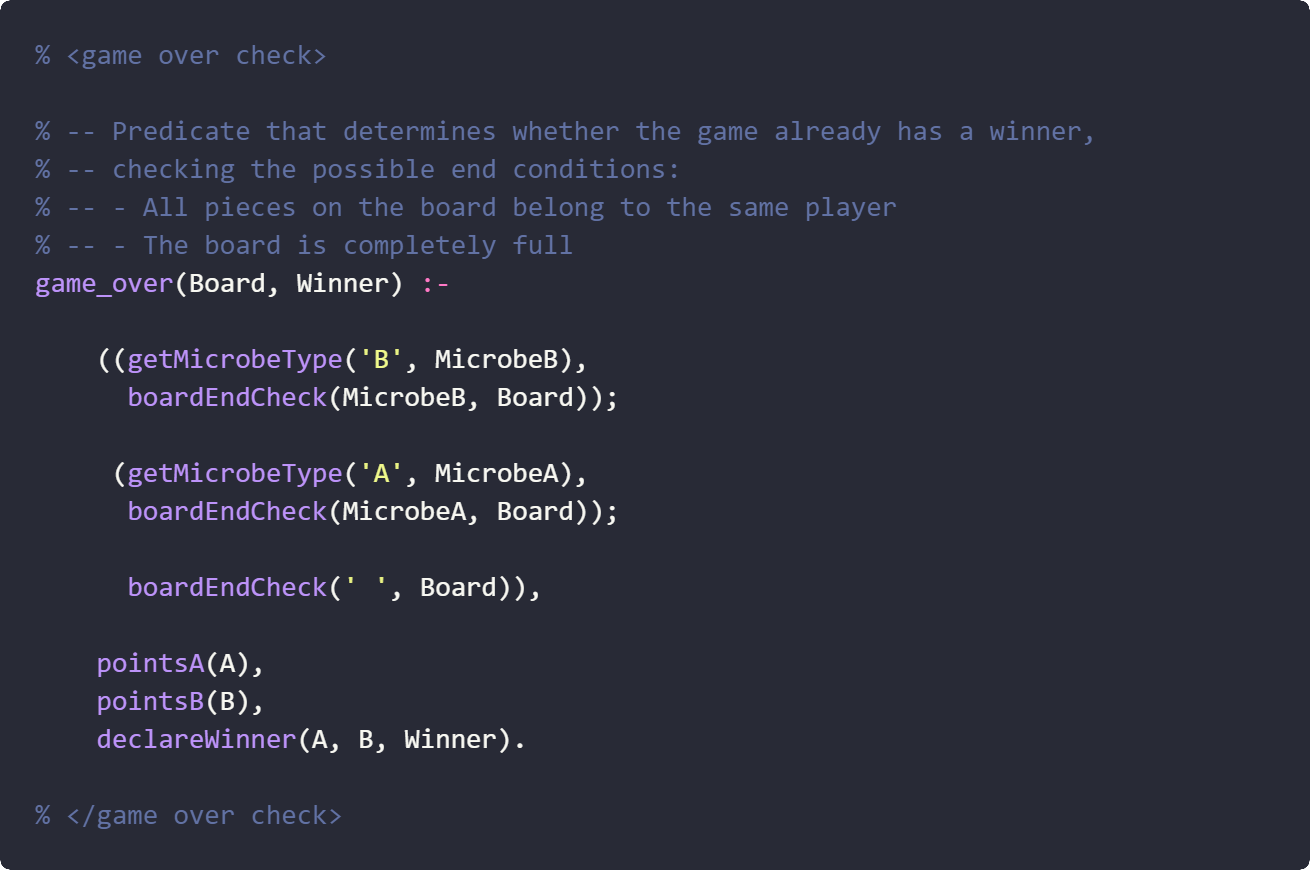
\includegraphics[width=\linewidth]{prints/game-over.png}
    \caption{Código que verifica e, se caso disso, executa o final do jogo}
    \label{fig}
\end{figure}

\begin{figure}[hbp!]
    \centering
    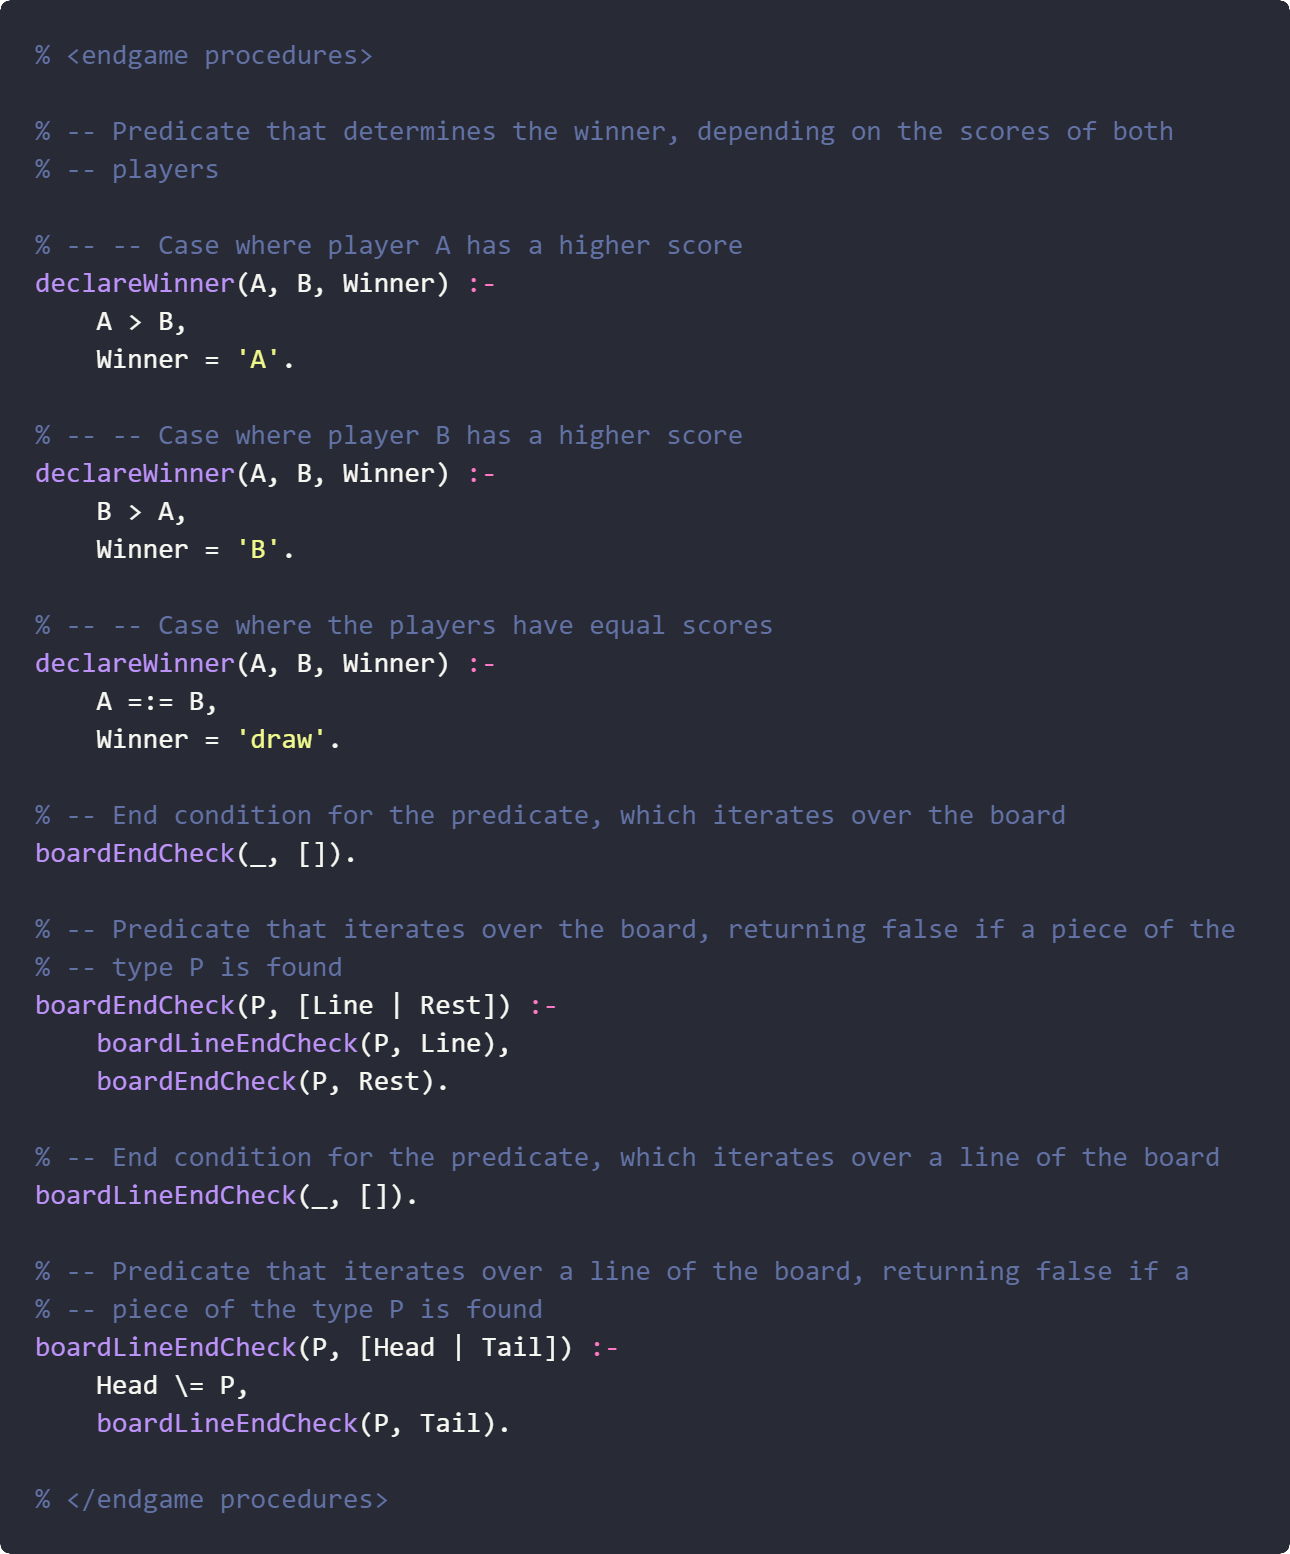
\includegraphics[width=\linewidth]{prints/game-over-check.png}
    \caption{Código auxiliar de final de jogo}
    \label{fig}
\end{figure}

\newpage\subsection{Avaliação do Tabuleiro (\textit{value})}

\bigskip
Este predicado avalia o estado de jogo que lhe é passado como argumento, através de \textbf{Board}, retornando em \textbf{Value} um valor inteiro que caracteriza o valor desse estado, sendo que quanto maior for esse valor, mais “vantajoso” é esse estado relativamente ao \textbf{Player} passado como argumento.

\bigskip
Optamos por desenvolver e integrar 2 níveis de dificuldade do “AI” do nosso jogo: easy (\textbf{nível 1}) e medium (\textbf{nível 2}). O predicado \textbf{value} apenas é chamado quando um computador se encontra no nível 2 de dificuldade (no nível 1 é gerado um value aleatório; irá ser visto mais à frente).

\bigskip
A função \textbf{value} retorna a diferença entre o número de peças do utilizador e o número de peças do oponente. É uma estratégia gananciosa que faz com que um computador a jogar no nível 2 escolha sempre a jogada que é mais vantajosa, nessa altura, para ele, uma vez que tendo uma lista de jogadas válidas, a jogada escolhida é a que adiciona mais peças do jogador ao tabuleiro e/ou a que retira mais peças do oponente.

\bigskip
\begin{figure}[hbp!]
    \centering
    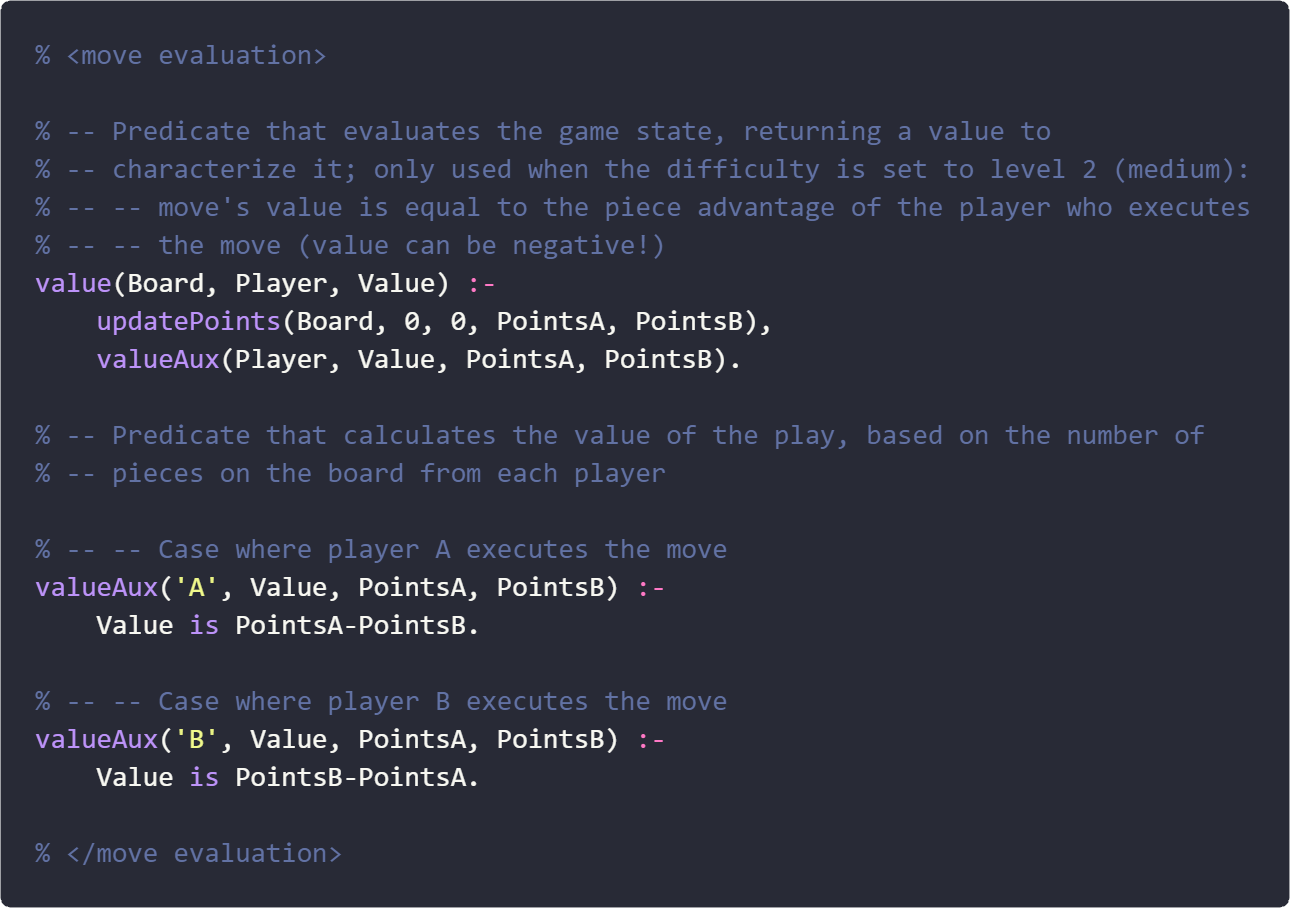
\includegraphics[width=\linewidth]{prints/move-evaluation.png}
    \caption{Predicado de avaliação do tabuleiro}
    \label{fig}
\end{figure}

\newpage\subsection{Jogada do Computador (\textit{choose\_move})} 

\bigskip
Este predicado apenas é chamado no turno de um computador, sendo que não é utilizado quando se trata de um humano a jogar. Este gera todos os possíveis movimentos/jogadas que o computador pode fazer, através de \textbf{valid\_moves}, e através de \textbf{chooseBestMove} avalia cada jogada, e retorna aquela que é considerada a melhor.

\bigskip
A maneira como as jogadas são avaliadas varia com o nível de dificuldade do computador que chama o predicado (passado em \textbf{Level}). 

\bigskip
Para o nível 1, e tal como foi dito anteriormente, a cada possível jogada irá ser atribuída um value aleatório, de 0 a 99 (números arbitrários, podiam ser outros), fazendo com que a jogada escolhida seja completamente aleatória. 

\bigskip	
Para o nível 2, cada jogada é “simulada”, sendo chamado o predicado move para construir o Board resultante da aplicação dessa jogada. Esse Board é então avaliado recorrendo à função \textbf{value} descrita anteriormente. Deste modo, a jogada retornada é a que está associada ao maior valor retornado por essa função \textbf{value}.

\bigskip
Se o jogador que invoca o predicado não tiver movimentos válidos que possa fazer (\textbf{valid\_moves} retorna uma lista vazia), então o movimento retornado é \textbf{movement(0, 0, 0, 0)}, o que indica a outro setor do código que o jogador não tem jogadas válidas e que o seu turno deverá ser passado à frente.

\bigskip
O predicado recebe como argumentos o \textbf{Level}, o \textbf{Player} que está a jogar, e o \textbf{Board} atual. Retorna o melhor movimento/jogada, em \textbf{movement(OldLine, OldColumn, NewLine, NewColumn)}.

\bigskip
\begin{figure}[hbp!]
    \centering
    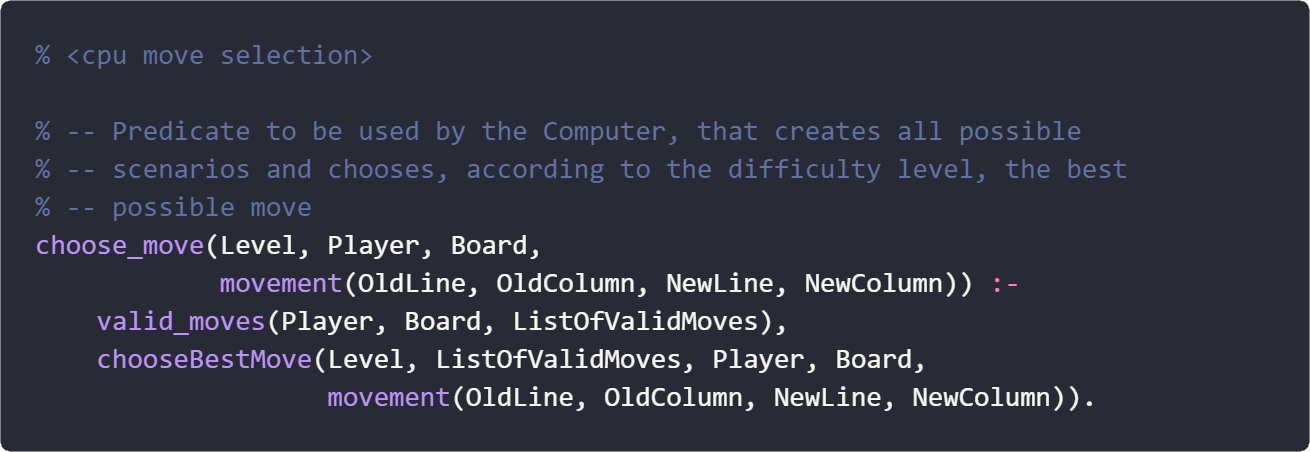
\includegraphics[width=\linewidth]{prints/move-selection-1.png}
    \caption{Predicado que selecciona a jogada do computador}
    \label{fig}
\end{figure}

\newpage
\begin{figure}[hbp!]
    \centering
    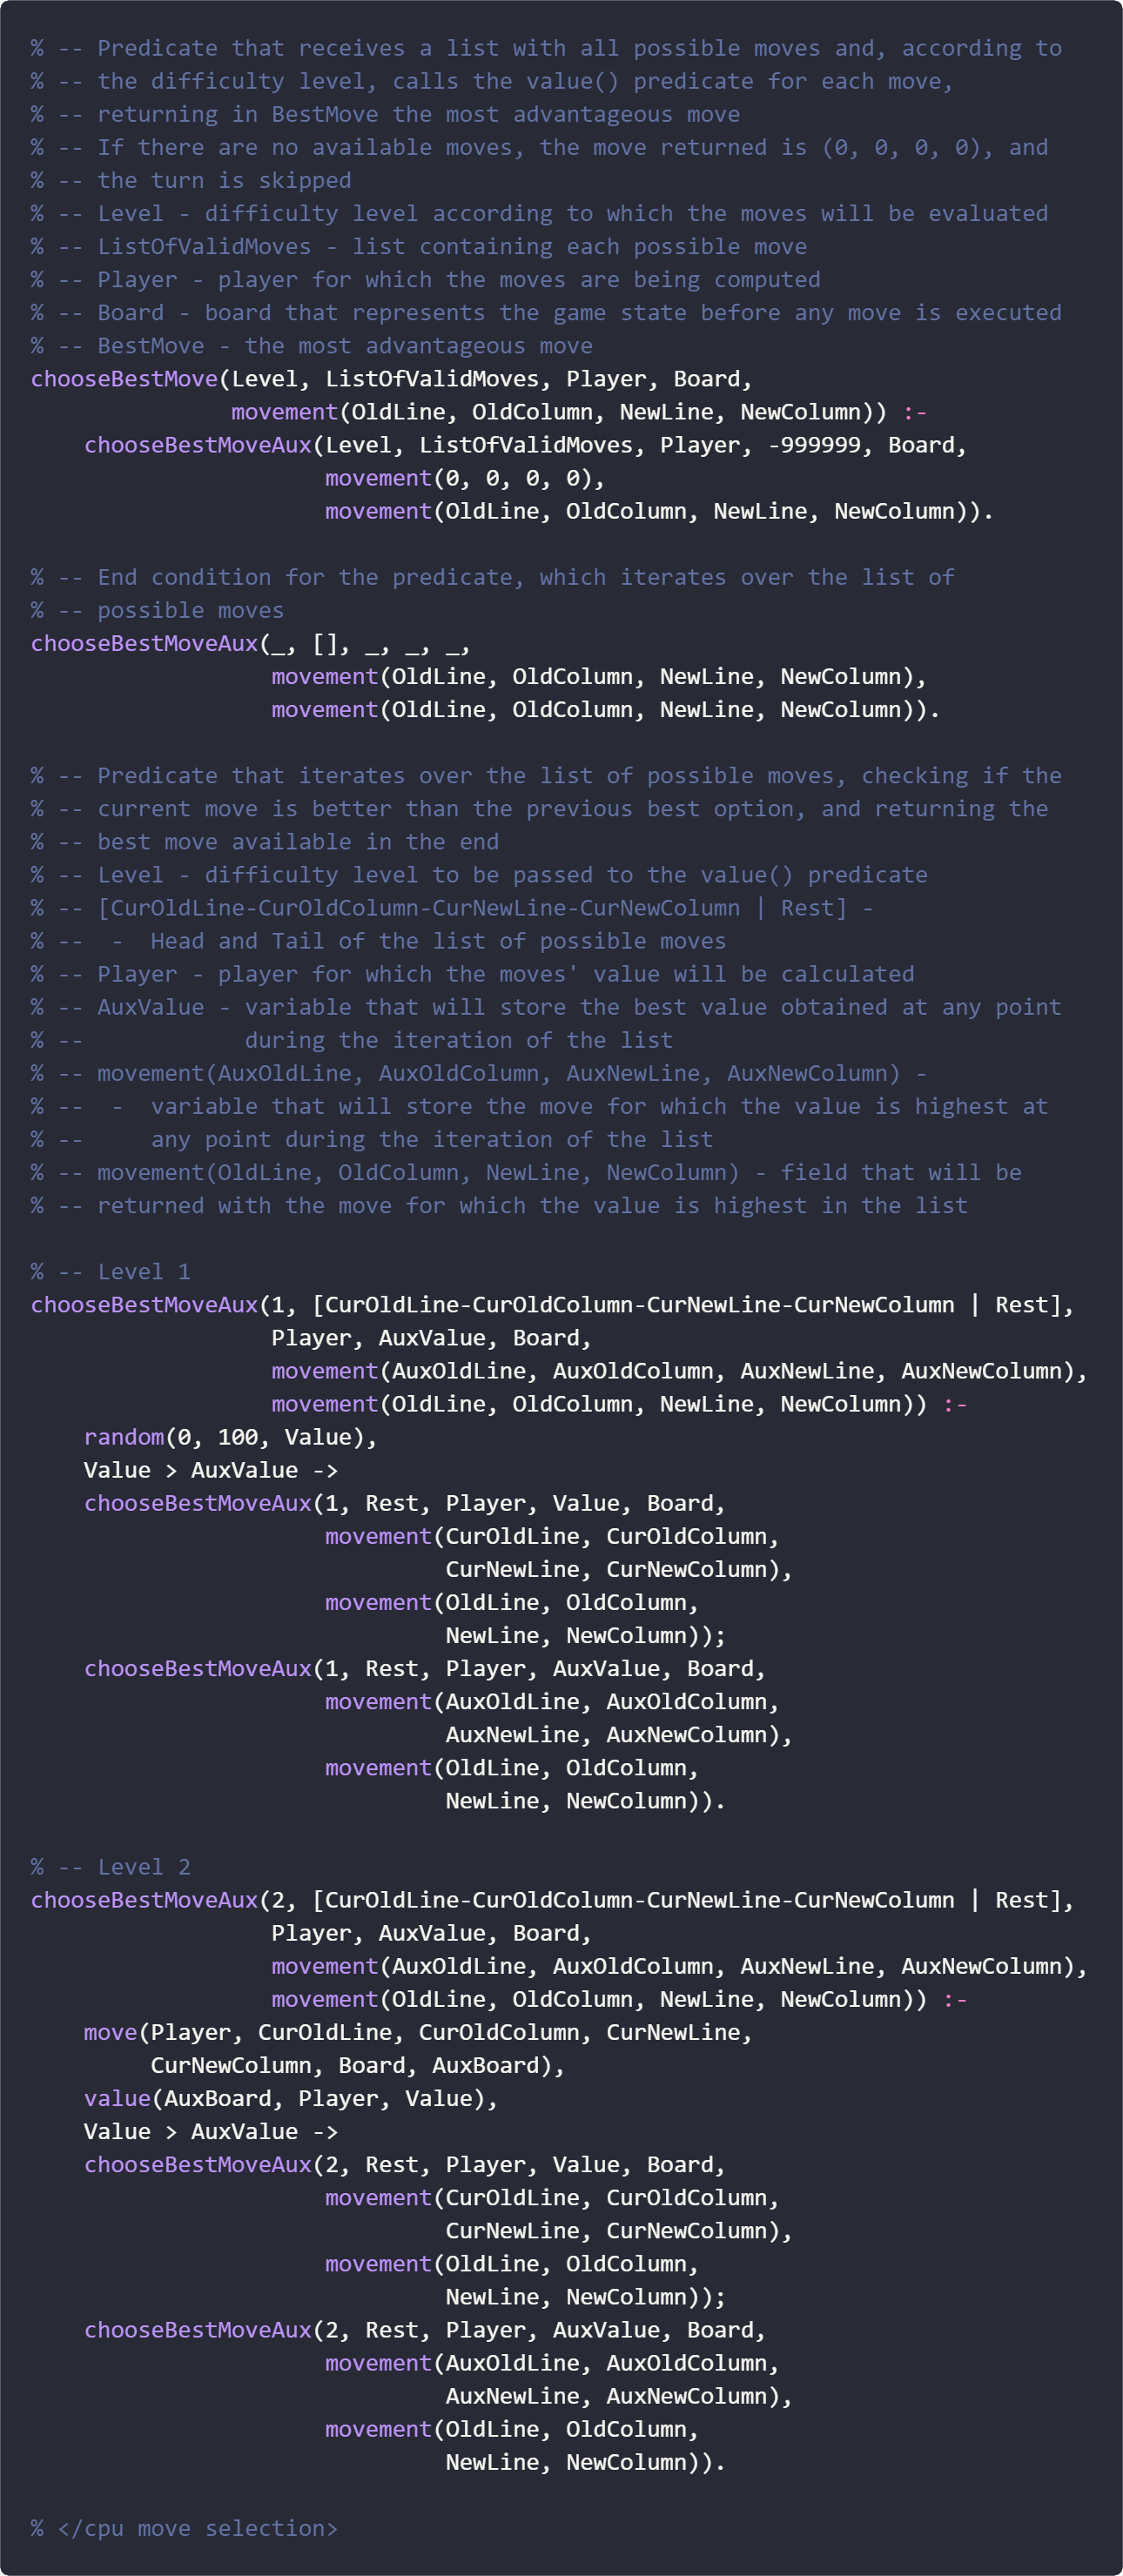
\includegraphics[width=.593\linewidth]{prints/move-selection-2.png}
    \caption{Código que selecciona a mais vantajosa das jogadas fornecidas}
    \label{fig}
\end{figure}

%%%%%%%%%%%%%%%%%%%%%%%%%%
\newpage\section{Conclusões}

\bigskip
O projeto teve como propósito a aplicação prática dos conhecimentos e competências adquiridas nas aulas teóricas e teorico-práticas da unidade curricular de Programação em Lógica, exigindo a formulação de todo o processo de pensamento do jogo adaptado às necessidades e características da linguagem \textit{Prolog}.

\bigskip
Ao longo do seu desenvolvimento, foram encontradas algumas dificuldades, como a questão de implementar os raciocínios formulados para a resolução de cada problema seguindo as normas da programação em Prolog, sendo uma característica marcante o uso quase constante da recursividade. No entanto, as dificuldades encontradas foram superadas pelo final do projeto.

\bigskip
Como seria de esperar, há aspetos do trabalho que poderiam ser melhorados. Um exemplo seria a implementação de um nível de inteligência artificial que seguisse uma estratégia superior à estratégia gananciosa que foi implementada, tendo possivelmente em conta as possíveis jogadas seguintes à calculada pelo computador. Além disto, seria também positivo otimizar o desempenho dos predicados desenvolvidos.

\bigskip
Concluindo, o trabalho foi concluído com sucesso, tendo contribuído para a aquisição e consolidação das competências pretendidas para a unidade curricular, e proporcionado uma boa aprendizagem da linguagem de programação \textit{Prolog}.

\newpage
\begin{thebibliography}{}

\bibitem{wikipedia}
    The 7th Guest: Infection,
    accessed on October of 2019,
    
    \url{https://en.wikipedia.org/wiki/The_7th_Guest:_Infection}.

\bibitem{boardgamegeek}
    The 7th Guest: Infection | Board Game,
    accessed on October of 2019.
    
    \url{https://www.boardgamegeek.com/boardgame/284017/7th-guest-infection}.

\bibitem{youtube}
    The 7th Guest Infection - iPad - US - Gameplay Trailer,
    
    \url{https://www.youtube.com/watch?v=4VheoiJdnUM}.
    
\bibitem{toucharcade}
    Eli Hodapp, for TouchArcade,
    27 April 2011,
    accessed on October of 2019,
    
    \url{https://toucharcade.com/2011/04/27/the-7th-guest-infection-for-ipad/}.

\end{thebibliography}

\end{document}
